\documentclass{article}
\usepackage[utf8]{inputenc}
\usepackage[allcolors=blue]{hyperref}
\usepackage[left=2.3cm, right=2.3cm, scale=0.75,top=2cm, bottom=2cm]{geometry}
\usepackage[all]{hypcap}
\usepackage{caption}
\usepackage{natbib} % Use natbib for citing
\usepackage{amsfonts}
\usepackage{amsmath}
\usepackage{graphicx} 
\usepackage{tikz}
\graphicspath{{../graphs/}}
\usetikzlibrary{patterns}




\title{Each period: 1 consumer, two producers}
\author{Iana Gerina}
\date{\today}
%\geometry{
% a4paper,
% left=20mm,
% top=15mm,
% right=20mm,
% bottom=15mm,
% }

\begin{document}

\maketitle


\section{$\alpha$ - probability of seeing the entrant}

As a basis we take the standard linear city Hotelling model, where consumers are distributed uniformly on (0,1). The supply side is reperesented by two producers: the entrant and the incumbent. While the incumbent is known to the consumers, the entrant first needs to be noticed by them. 

Assume in each period only 1 consumer is looking to buy the good. Let us denote $\alpha \in (0,1)$ as the probability of entrant being noticed. Then, there are two states of the world in each period:

\begin{itemize}
    \item with probability $\alpha$ we arrive at state 1: duopoly, the demand that the producers face is reminiscent of standard Hotelling model;
    \item with probability $1-\alpha$ we arrive at state 2: monopoly, where consumer obly sees the incumbent.
\end{itemize}

Suppose we have a one-preiod game. Then if $\alpha = 0$ the incumbent is always a monopolist. What is the pricing strategy under monopoly? The incumbent solves:
$$\max_{p^{inc}} (p^{inc}-c)* Pr(p^{inc}\leq v-t*x)$$

The demand the monopoly faces is then $\frac{v-p^{inc}}{t}$ as $Pr(p^{inc}\leq v-t*x) = Pr(x\leq \frac{v-p^{inc}}{t})$, the optimal price of the monopolist is $p_inc = v/2 $ and his profit is $\tfrac{v^2}{4t}$.

If, on the other hand, $\alpha=1$, the game is basically the standard linear city model with duopoly. The demands that incumbent and entrant face are, in same order:
$$ x =  \tfrac{p^{e}_2 - p^{inc}_2}{2t} + 1/2 $$
$$1-x = \tfrac{p^{inc}_2 - p^{e}_2}{2t} + 1/2$$

No we will exapnd the model to encompass two periods. The information structure is as follows: the probability of entrant being seen is known to both entrant and incumbent, and so is the event of entrant being noticed. Until that point both producers assume he was not and assign probability $\alpha$ to that event happening in each period. If consumer gets noticed in the first period, $\alpha =1$ in the second period.To simplify matters further, let us assume c=0 for both producers. We start from the second period.

As was mentioned above, we have two possible states: if entrant was noticed in the first period and if he wasn't. If \textbf{entrant was noticed}, the solution is straightforward, as it is the prices, demands and profits of standard Hotelling duopoly, that we already established. The equilibrium prices are then: $p^{inc}_2 = p^{e}_2 = t+c$ and as we establichd c=0, the price is then just equal to transportation cost. The profits in this case are 1/2t for each of the firms.

However, if the \textbf{entrant was not noticed}, the solution is less straightforward. With probability $\alpha$ the state is a duopoly with corresoonding duopolistic demands that the producers face and with probability $1- \alpha$ it's a monopoly with corresponding demand described above. 
The expected profits in the second period that they maximise are then:

$$ \pi^{inc}_2 = p_2^{inc}*((1-\alpha)Pr(x \leq \tfrac{v-p_2^{inc}}{t}) +  \alpha(Pr(x \leq \tfrac{p^{e}_2 - p^{inc}_2}{2t}) + 1/2)$$

$$ \pi^{e}_2 = \alpha *p_2^{e}(Pr(x > \tfrac{p^{e}_2 - p^{inc}_2}{2t}) + 1/2)
$$

Solving for optimal price we get:

$$
p_2^{inc} = \tfrac{3\alpha t}{8-5\alpha} + \tfrac{4(1-\alpha)v}{8-5\alpha}$$
$$
p_2^{e} = \tfrac{(4-\alpha)t}{8-5\alpha} + \tfrac{2(1-\alpha)v}{8-5\alpha}
$$

Notice that for $\alpha = 1$ the prices of both incumbent and entrant are our duopoly prices from one-period game and for $\alpha=0$ the price of incumbent is the monopoly price. 
Substituting optimal prices into the profit equation we get: 

$$ \pi^{inc}_2 = \tfrac{2-\alpha}{2t}(\tfrac{4v(1-\alpha) + 3\alpha t}{8-5\alpha})^2$$

$$ \pi^{e}_2 = \tfrac{\alpha}{2t}(\tfrac{(4-\alpha)t}{8-5\alpha} + \tfrac{2(1-\alpha)v}{8-5\alpha})^2
$$
Notice that for $\alpha=0$ the profit of entrant is 0 and the profit of incumbent is the monopolist profit $\tfrac{v^2}{4t}$ and for $\alpha=1$ the profits are again the dupoly profits $1/2t$ for both producers.

Discounted sums of profits in the first period for both producers can be then written as:

 $$ \pi^{inc} = (1-\alpha)(\frac{v-p_1^{inc}}{t}*p_1^{inc}) +  \alpha(\tfrac{p^{e}_1 - p^{inc}_1}{2t} + 1/2)p^{inc}_1) + \beta(\alpha(\tfrac{p^{e}_2 - p^{inc}_2}{2t} + 1/2)p^{inc}_2 +(1-\alpha)(p_2^{inc}*\tfrac{v-p_2^{inc}}{t}))  $$
   
 $$ \pi^{e} = \alpha_1(\tfrac{p^{inc}_1 - p^{e}_1}{2t} + 1/2)(p^{e}_1 -c) + \beta(\alpha_2(\frac{p^{e}_2 - p^{inc}_2}{2t} + 1/2))(p^{e}_2 -c)  $$

where $\alpha_2 = \alpha(1-\alpha)+\alpha$

It's quite evident from both expressions that profit maximisation in both periods is independent of each other and in fundamentals similar, so we can look for optimal strategies in the first period and then approximate for the next one.

Best responses are then:

$$ p^{e}_t = \frac{c+p^{inc}+t}{2}$$
$$ p^{inc}_t = \frac{(c+v)(1-\alpha_t)}{2-\alpha_t} + \frac{\alpha_t}{2-\alpha_t}*\frac{c+p_t^{e}}{2} + \frac{\alpha_t}{2(2-\alpha_t)}, $$
for $t \in {1,2}$.

The prices evolve over time only via the evolution of $\alpha_t$, which becomes closer and closer to 1 with each time period.

\section{Perceived [0,y] linear city}
Assume we have two producers on the market: one is incumbent and one is entrant. Suppose location of incumbent and entrant is set: 0 for incumbent and 1 for entrant, however, the consumer perceives the location of entrant as $y>1$ in the first period. The strategies of the producers are then prices: $p_{inc}$ and $p_{e}$ - price of incumbent and entrant respectively. Consumer chooses between the option offered by the incumbent and the entrant (and an outside option, whose value we set to 0), and if in the first period the entrant is chosen, his true location is revealed to the consumer in the second period.

As the original model talks about a set of consumers, whose tastes are distributed uniformly on [0,1], our model's one consumer setting leads to a different demand estimation technique. If v is consumer's valuation of the object and x is his location, which is a random draw from U[0,1], then his utility is:

    $$ U = \begin{cases}
    v - t*x - p_{inc} &  \text{if } v-t*x - p_{inc} \geq v - t(y-x) - p_{e}\\
    v - t*x - p_{e} &  \text{if } v-t*x - p_{inc} < v - t(y-x) - p_{e}
    \end{cases}
$$

Then, demand for incumbent's good is:

$$d_{inc} = \begin{cases}
    1 &  \text{if } x \leq \frac{p_{e}-p_{inc}}{2t} + 1/2y\\
    0 &  \text{if } x > \frac{p_{e}-p_{inc}}{2t} + 1/2y
    \end{cases}
$$
 and vice versus for demand of the entrant.
 
In a one period game incumbent then solves:
$$\max_{p^{inc}} (p^{inc}-c)* Pr(x \leq \frac{p_{e}-p_{inc}}{2t} + 1/2y),$$
which can be simplified to:
$$\max_{p^{inc}} (p^{inc}-c)(\frac{p_{e}-p_{inc}}{2t} + 1/2y)$$
and entrant's profit-maximising problem to:
$$\max_{p^{e}} (p^{e}-c)(\frac{p_{inc}-p_{e}}{2t} + 1 - 1/2y)$$

\subsection{Random consumer location}
    
    Suppose we only have one consumer, who is located differently in each period (random draw from U[0,1]). Once consumer is located s.t. the entrant's good is his best option, in the next periods he perceives the true location of the entrant.
    
    Suppose we have a two-period game. Then from the first period point of view, the probability of the entrant being seen in the second period depends on the probability of him being the best option in the first period. Thus, we can write the optimization problem in the first period for both incumbent and entrant as follows:
    
    $$ \begin{aligned}
    \max_{p^{inc}_1, p^{inc}_2} {}
    & \quad (p^{inc}_1-c)* Pr(x_1 \leq \frac{p^{e}_1-p^{inc}_1}{2t} + 1/2y) + \\
    & \quad + \beta((p^{inc}_2-c)(Pr(x_1 \leq \frac{p^{e}_1-p^{inc}_1}{2t} + 1/2y)(Pr(x_2 \leq \frac{p^{e}_2-p^{inc}_2}{2t} + 1/2y)) + \\
    & \quad + (Pr(x_1 > \frac{p^{e}_1-p^{inc}_1}{2t} + 1/2y))(Pr(x_2 \leq \frac{p^{e}_2-p^{inc}_2}{2t} + 1/2)))
    \end{aligned}
    $$

    $$ \begin{aligned}
    \max_{p^{e}_1, p^{e}_2} {}
    & \quad (p^{e}_1-c)* Pr(x_1 > \frac{p^{e}_1-p^{inc}_1}{2t} + 1/2y) + \\
    & \quad + \beta((p^{e}_2-c)(Pr(x_1 \leq \frac{p^{e}_1-p^{inc}_1}{2t} + 1/2y)(Pr(x_2 \leq \frac{p^{inc}_2-p^{e}_2}{2t} + 1 - 1/2y)) + \\
    & \quad + (Pr(x_1 > \frac{p^{e}_1-p^{inc}_1}{2t} + 1/2y))(Pr(x_2 \leq \frac{p^{inc}_2-p^{e}_2}{2t} + 1/2))),
    \end{aligned}
    $$
where $x_1$, $x_2$ are locations of the consumer in each period. 

    
Solving by backward induction, we first discuss the equilibrium conditions in the second period. 
If entrant is noticed, the solution corresponds to classic Hotelling and the profit is then standard $\pi_{2}^{inc} = \pi_{2}^{e}= t/2$. However, if entrant is not noticed, equilibrium prices are as follows:
$$
p^{inc}_2 =1/3t(y+ 2) + c $$
$$ p^{e}_2 =4/3t - 1/3yt + c$$
To make sure that the profits don't go into the negative values, $ p^{e}_2$ should be less than 4, otherwise entrant does not enter the market. Then the profits are $\pi_{2}^{e} = 1/18*t(4-y)^2$ and $\pi_{2}^{inc}=1/18*t(2+y)^2$, respectively. The profit of incumbent is increasing in y and the profit of entrant is decreasing in y for all the allowed values of y ($1<y\leq4$), exponentially. Also notice that if y=1, the profits equations collapse to the classic Hotelling profits. 

Now each producer optimizes their behaviour in the first period, assuming that in each state (multiplied by corresponding probability of reaching it) in the second period they will behave optimally. 

	


 $$
    \max_{p^{inc}_1} {}
   (p^{inc}_1-c)(\frac{p^{e}_1-p^{inc}_1}{2t} + 1/2y) 
    + \beta((\frac{p^{e}_1-p^{inc}_1}{2t} + 1/2y)(\frac{1}{18}t(2+y)^2) + 
    1/2t(\frac{p^{inc}_1-p^{e}_1}{2t} + 1 - 1/2y))
    $$
    
    $$
   \max_{p^{e}_1} {}
   (p^{e}_1-c)(\frac{p^{inc}_1-p^{e}_1}{2t} + 1 -1/2y) 
    + \beta((\frac{p^{e}_1-p^{inc}_1}{2t} + 1/2y)(\frac{1}{18}t(4-y)^2) + 
    1/2t(\frac{p^{inc}_1-p^{e}_1}{2t} + 1 - 1/2y))
    $$

The equilibrium prices in the first period are then:
$$
p^{inc}_1 =1/3t(y+ 2) + c - \frac{\beta t }{54}(y-1)(17+y) $$
$$ p^{e}_1 =4/3t - 1/3yt + c - \frac{\beta t}{54}(y-1)(19-y)$$
Notice that for both the prices the RHS until the $ \beta$ component correspond to our second period equilibrium, the 'unnoticed entrant' state, which in turn collapses to the standard result, when y=1. There is also no dynamic effect in the price, if y=1, as the component becomes 0 - also quite logical, as the dynamic effect appears because of the difference between two states' profits in the second period. From the first equation we can see that the dynamic effect always brings the price of incumbent in the first period down, for any value of $y>1$, which makes sense, as the higher value of y makes the gap between two states' profits for the incumbent in the second period bigger. The marginal effect, interestingly, increases with y. The price of incumbent is also decreasing with the dynamic component, however, the shape of the component is convex. You can see on the graph, that for the allowed values of y the functions almost coincide, the closer y is to 1, the closer the lines come together. I can't, however, come up with a good intuition, as to why this difference in shape occurs at all and will look into the calculations for possible arithmetic mistakes. However, also notice that the part of the price corresponding to maximisation of profit in the first period has price increasing with y for incumbent and decreasing with y for entrant.


\begin{center}
    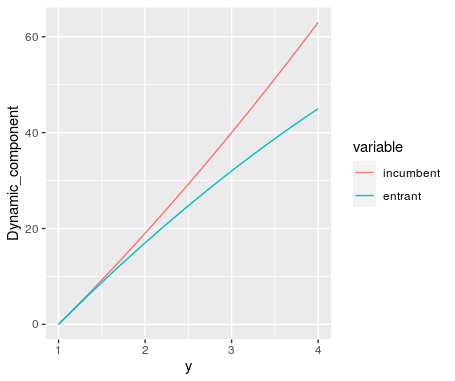
\includegraphics[scale=0.5]{dynamiccomponent.png}
\end{center}



\subsection{Fixed consumer location}

Assume now that location of consumer is fixed and in the second period, partially revealed via his choice of the product. Indeed, if the consumer chooses the entrant, in second period both producers know, that:
$p_1^{inc}+t*x>p_1^{e}+t(y-x)$. And since the prices of the first period are revealed by the second period and t is constant, the location x becomes clearer to both producers. It makes the second period interaction a bit more interesting, as now both the producers have additional information. 

We'll start again with the second period. Suppose \textbf{the entrant was chosen}. Then we know that $p_1^{inc}+t*x>p_1^{e}+t(y-x)$. Let us denote $ \frac{p_2^{e}-p_2^{inc}}{2t}+1/2$ as f and $\frac{p_1^{e}-p_1^{inc}}{2t}+y/2$ as e. For the incumbent the probability of selling the good to the consumer in second period, if entrant is noticed, equals: $Pr(x<\frac{p_2^{e}-p_2^{inc}}{2t}+1/2 | x > \frac{p_1^{e}-p_1^{inc}}{2t}+y/2) = Pr(x<f|x>e)$, and for the entrant it is equal: $ Pr(x>\frac{p_2^{e}-p_2^{inc}}{2t}+1/2 | x >\frac{p_1^{e}-p_1^{inc}}{2t}+y/2 = Pr(x>f|x>e)$.
Evidently, the first period interaction results in two separate outcomes for different values of f and e. Suppose this condition holds:

$$ \frac{p_2^{e}-p_2^{inc}}{2t}+1/2 > \frac{p_1^{e}-p_1^{inc}}{2t}+y/2,$$
meaning \pmb{$f>e$}. We denote with red colour the condition on e and with blue the condition on f. 

%new ind cons to the left.
\begin{tikzpicture}
    % entrant 
    
    \draw[step=0.4cm,gray,very thin] (-2,-1) grid (3.6,2) node[anchor=north east, black] {entrant};
    \draw[thick] (-1.6,0) -- (2.4,0);
    \draw[thick, ->] (-1.6,0) -- (-1.6,1.6);
    \draw (-1.55,0.8) -- (-1.65,0.8) node[anchor=east] {1};
    \draw[thick, dashed] (2.4,0) -- (3.2,0);
    \draw (-1.6,1pt) -- (-1.6,-1pt) node[anchor=north] {0};
    \draw (2.4,1pt) -- (2.4,-1pt) node[anchor=north] {1};
    \draw (3.2,1pt) -- (3.2,-1pt) node[anchor=north] {y};
    \draw (1.2,1pt) -- (1.2,-1pt) node[anchor=north] {f};
    \draw[label distance=10mm] (0,1pt) -- (0,-1pt) node[anchor=north] {e};
    \draw[pattern=north east lines, pattern color=red] (0,0) rectangle (2.4,0.8);
    \draw[pattern=north west lines, pattern color=blue] (1.2,0) rectangle (2.4,0.8);

    % incumbent
    
    \draw[step=0.4cm,gray,very thin] (6.4,-1) grid (12,2) node[anchor=north east, black] {incumbent};
    \draw[thick] (6.8,0) -- (10.8,0);
    \draw[thick, dashed] (10.8,0) -- (11.6,0);
    \draw[thick, ->] (6.8,0) -- (6.8,1.6);
    \draw (6.75,0.8) -- (6.85,0.8) node[anchor=east] {1};
    \draw (6.8,1pt) -- (6.8,-1pt) node[anchor=north] {0};
    \draw (10.8,1pt) -- (10.8,-1pt) node[anchor=north] {1};
    \draw (11.6,1pt) -- (11.6,-1pt) node[anchor=north] {y};
    \draw (8.4,1pt) -- (8.4,-1pt) node[anchor=north] {e};
    \draw (9.6,1pt) -- (9.6,-1pt) node[anchor=north] {f};
    \draw[pattern=north east lines, pattern color=blue] (6.8,0) rectangle (9.6,0.8);
    \draw[pattern=north west lines, pattern color=red] (8.4,0) rectangle (10.8,0.8);
    

\end{tikzpicture}

From the graph we see that the demand the entrant faces is equal to $Pr(x>f|x>e)=\frac{1-f}{1-e}$. Demand of the incumbent, on the other hand, is is equal to $Pr(x \leq f| x >e) = \frac{f-e}{1-e}$. Substituting these equations into the corresponding profit functions and solving for optimal price, we derive the following equilibrium prices:
$$ p_2^{inc} = t+c+ 2/3(p_1^{inc}-p_1^{e}-yt)$$
$$ p_2^{e} = t+c + 1/3(p_1^{inc}-p_1^{e}-yt),$$
for all $p_1^{inc}$, $p_1^{e}$ s.t. $p_1^{inc}-p_1^{e}+(2-y)t \neq 0$.

$p=t+c$ is a standard Hotelling result. The new term of the price can be both negative and positive, which is not easy to pinpoint. As we assumed the entrant was chosen in the first period, we know that $p_1^{inc}-p_1^{e}-yt>-2tx$. Then it can take negative values from the interval $(-2tx,0)$ and any positive values. Using the expressions for the price from higher above, we derive equilibrium profits for both incumbent and entrant, should this outcome occur:
$$\pi_2^{inc} = \frac{(t+2/3(p_1^{inc}-p_1^{e}-yt))^2}{p_1^{inc}-p_1^{e}+(2-y)t} $$
$$\pi_2^{e} = \frac{(t+1/3(p_1^{inc}-p_1^{e}-yt))^2}{p_1^{inc}-p_1^{e}+(2-y)t} $$
Note that both cases are possible: that profit of incumbent is higher than profit of entrant, and vice versus.


If, however, \pmb{$f\leq e$}, the situation is quite different. 

\begin{tikzpicture}
    % entrant 
    
    \draw[step=0.4cm,gray,very thin] (-2,-1) grid (3.6,2) node[anchor=north east, black] {entrant};
    \draw[thick] (-1.6,0) -- (2.4,0);
    \draw[thick, ->] (-1.6,0) -- (-1.6,1.6);
    \draw (6.75,0.8) -- (6.85,0.8) node[anchor=east] {1};
    \draw (-1.55,0.8) -- (-1.65,0.8) node[anchor=east] {1};
    \draw[thick, dashed] (2.4,0) -- (3.2,0);
    \draw (-1.6,1pt) -- (-1.6,-1pt) node[anchor=north] {0};
    \draw (2.4,1pt) -- (2.4,-1pt) node[anchor=north] {1};
    \draw (3.2,1pt) -- (3.2,-1pt) node[anchor=north] {y};
    \draw (1.2,1pt) -- (1.2,-1pt) node[anchor=north] {e};
    \draw (0,1pt) -- (0,-1pt) node[anchor=north] {f};
	\draw[pattern=north east lines, pattern color=blue] (0,0) rectangle (2.4,0.8);
    \draw[pattern=north west lines, pattern color=red] (1.2,0) rectangle (2.4,0.8);
    
    
    
    % incumbent
    
    \draw[step=0.4cm, gray, very thin] (6.4,-1) grid (12,2) node[anchor=north east, black] {incumbent};
    \draw[thick] (6.8,0) -- (10.8,0);
    \draw[thick, ->] (6.8,0) -- (6.8,1.6);
     \draw[thick, dashed] (10.8,0) -- (11.6,0);
    \draw (6.8,1pt) -- (6.8,-1pt) node[anchor=north] {0};
    \draw (6.75,0.8) -- (6.85,0.8) node[anchor=east] {1};
    \draw (10.8,1pt) -- (10.8,-1pt) node[anchor=north] {1};
    \draw (11.6,1pt) -- (11.6,-1pt) node[anchor=north] {y};
    \draw (8.4,1pt) -- (8.4,-1pt) node[anchor=north] {f};
    \draw (9.6,1pt) -- (9.6,-1pt) node[anchor=north] {e};
    \draw[pattern=north east lines, pattern color=blue] (6.8,0) rectangle (8.4,0.8);
    \draw[pattern=north west lines, pattern color=red] (9.6,0) rectangle (10.8,0.8);

\end{tikzpicture}
    
As both producers know for sure that $x>f$, in the second case entrant sells his good with probability 1, whereas the incumbent does not sell.
Then the entrant puts the price as high as he can, without running off the consumer, i.e. keeping $f\leq e$. That denotes a whole set of possible solutions, where prices of both incumbent and entrant are compliant with this condition and the consumer's participation constraint $v-p^{inc}_2-t(1-x)>0$. As far as I understand, the equilibrium prices are not among them, as f depends on both the incumbent's and entrant's price. The entrant wants to put the price as high as possible, however, the incumbent answers that action with decreasing his price until $f>e$ again as for him it is the only way to gain profit. Is it possible for the entrant to set such a price so as to block the incumbent from entering the market? The lowest possible price he can set is $p^{e}_2 = c$. Suppose he sets the price c, then the incumbent's price needed to keep the equilibrium in $f\leq e$ should be bigger or equal $c+p^{inc}_1-p^{e}_1 + t(1-y)$. Then suppose the incumbent also sets the price as low as possible. Then the condition for the entrant taking all of the market (i.e. attracting the consumer) is $p^{inc}_1-p^{e}_1 - t(y-1) \leq 0$. If y=1, then this condition is simply $p^{inc}_1 \leq p^{e}_1$; and any $y>1$ actually make the condition hold with less of a gap between two prices. This makes sense as this condition is simply that e, the expected indifferent consumer location from the first period, is closer to 1, which implies, since the entrant was chosen nonetheless, that x itself is much closer to entrant than incumbent. In this case the incumbent can't actually attract the consumer as it would require setting their price lower than c. The entrant, on the other hand, can actually increase their price by up to $|p^{inc}_1 - p^{e}_1 - t(y-1)|$ as long as the value under the modulus sign is negative. Notice also that from the intuition above solution inside the $f\leq e$ case is only possible if $p^{inc}_1 - p^{e}_1 - t(y-1) \leq 0$ holds.

Then the equilibrium is:
$$p^{e}_2  =  c - p^{inc}_1 + p^{e}_1 + t(y-1) 
$$
$$p^{inc}_2 \in (c, \infty)$$

and the profit of incumbent is always 0, where
as $\pi^{e}_2 = p^{e}_1 - p^{inc}_1 + t(y-1)$. Interestingly enough, the profit of entrant increases with y.
 


If \textbf{entrant is not chosen} in the first period, the situation is almost symmetric. Now both producers know that $p_1^{inc}+t*x \leq p_1^{e}+t(y-x)$, meaning that $x \leq \frac{p_1^{e}-p_1^{inc}+yt}{2t}$. Let us denote $\frac{p_2^{e}-p_2^{inc}}{2t}+y/2$ as d and keep the notation for e from previous section. As the entrant was not seen, the consumer chooses incumbent in the second period if $Pr(x \leq \frac{p_2^{e}-p_2^{inc}}{2t}+y/2 | p_1^{inc}+t*x \leq p_1^{e}+t(y-x)) = Pr(x \leq d | x \leq e)$ and the entrant if $Pr(x > \frac{p_2^{e}-p_2^{inc}}{2t}+y/2 | p_1^{inc}+t*x \leq p_1^{e}+t(y-x)) = Pr(x > d| x \leq e)$.  Then we have yet again two cases: when $d \geq e$ and $e<d$. We denote again with red colour the condition on e and with blue colour the condition on d.

Let's look at some illustrations for $d \geq e$.

\begin{tikzpicture}
   % entrant 
    
    \draw[step=0.4cm,gray,very thin] (-2,-1) grid (3.6,2) node[anchor=north east, black] {entrant};
    \draw[thick] (-1.6,0) -- (2.4,0);
    \draw[thick, ->] (-1.6,0) -- (-1.6,1.6);
    \draw (-1.55,0.8) -- (-1.65,0.8) node[anchor=east] {1};
    
    \draw[thick, dashed] (2.4,0) -- (3.2,0);
    \draw (-1.6,1pt) -- (-1.6,-1pt) node[anchor=north] {0};
    \draw (2.4,1pt) -- (2.4,-1pt) node[anchor=north] {1};
    \draw (3.2,1pt) -- (3.2,-1pt) node[anchor=north] {y};
    \draw (1.2,1pt) -- (1.2,-1pt) node[anchor=north] {d};
    \draw[label distance=10mm] (0,1pt) -- (0,-1pt) node[anchor=north] {e};
    \draw[pattern=north east lines, pattern color=red] (-1.6,0) rectangle (0,0.8);
    \draw[pattern=north west lines, pattern color=blue] (1.2,0) rectangle (2.4,0.8);

    % incumbent
    
    \draw[step=0.4cm,gray,very thin] (6.4,-1) grid (12,2) node[anchor=north east, black] {incumbent};
    \draw[thick] (6.8,0) -- (10.8,0);
    \draw[thick, ->] (6.8,0) -- (6.8,1.6);
    \draw (6.75,0.8) -- (6.85,0.8) node[anchor=east] {1};
    \draw[thick, dashed] (10.8,0) -- (11.6,0);
    \draw (6.8,1pt) -- (6.8,-1pt) node[anchor=north] {0};
    \draw (10.8,1pt) -- (10.8,-1pt) node[anchor=north] {1};
    \draw (11.6,1pt) -- (11.6,-1pt) node[anchor=north] {y};
    \draw (8.4,1pt) -- (8.4,-1pt) node[anchor=north] {e};
    \draw (9.6,1pt) -- (9.6,-1pt) node[anchor=north] {d};
    \draw[pattern=north east lines, pattern color=red] (6.8,0) rectangle (8.4,0.8);
    \draw[pattern=north west lines, pattern color=blue] (6.8,0) rectangle (9.6,0.8);
    

\end{tikzpicture}

Notice that for $d \geq e$ entrant has no chance of attracting the consumer, whereas the incumbent always does. Let's try our intuition from the previous section. The optimal price for the incumbent would have been the one, under which d=e, as the $d \geq e$ is obviously beneficial to the entrant and the higher the price, the bigger are the profits. However, incumbent can always move d away from this point into $d < e$ territory, where he has a non-zero probability to attract the consumer by lowering his own price. Can incumbent set a price s.t. entrant can no longer hinder him? Suppose entrant sets the price c, and since in this case the transportation cost part of the price actually cancels itself, we have: $ p_2^{inc}-c \leq p_1^{inc}-p_1^{e}$. So the maximal markup that the entrant can afford while keeping the consumer to himself is equal to $p_1^{inc}-p_1^{e}$, as long as $p_1^{inc} \geq p_1^{e}$. Similar to the previous case the optimal strategies are then:

Then the equilibrium is:
$$p^{inc}_2  =  c + p^{inc}_1 - p^{e}_1 
$$
$$p^{e}_2 \in (c, \infty)$$

and the profit of incumbent is always 0, whereas $\pi^{inc}_2 = p^{inc}_1  - p^{e}_1$. 

If $d < e$, however, the field is a bit more even.

\begin{tikzpicture}
   % entrant 
    
    \draw[step=0.4cm,gray,very thin] (-2,-1) grid (3.6,2) node[anchor=north east, black] {entrant};
    \draw[thick] (-1.6,0) -- (2.4,0);
    \draw[thick, dashed] (2.4,0) -- (3.2,0);
    \draw[thick, ->] (-1.6,0) -- (-1.6,1.6);
    \draw (-1.55,0.8) -- (-1.65,0.8) node[anchor=east] {1};
    \draw (-1.6,1pt) -- (-1.6,-1pt) node[anchor=north] {0};
    \draw (2.4,1pt) -- (2.4,-1pt) node[anchor=north] {1};
    \draw (3.2,1pt) -- (3.2,-1pt) node[anchor=north] {y};
    \draw (1.2,1pt) -- (1.2,-1pt) node[anchor=north] {e};
    \draw[label distance=10mm] (0,1pt) -- (0,-1pt) node[anchor=north] {d};
    \draw[pattern=north east lines, pattern color=red] (-1.6,0) rectangle (1.2,0.8);
    \draw[pattern=north west lines, pattern color=blue] (0,0) rectangle (2.4,0.8);

    % incumbent
    
    \draw[step=0.4cm,gray,very thin] (6.4,-1) grid (12,2) node[anchor=north east, black] {incumbent};
    \draw[thick] (6.8,0) -- (10.8,0);
    \draw[thick, ->] (6.8,0) -- (6.8,1.6);
    \draw (6.75,0.8) -- (6.85,0.8) node[anchor=east] {1};
    \draw[thick, dashed] (10.8,0) -- (11.6,0);
    \draw (6.8,1pt) -- (6.8,-1pt) node[anchor=north] {0};
    \draw (10.8,1pt) -- (10.8,-1pt) node[anchor=north] {1};
    \draw (11.6,1pt) -- (11.6,-1pt) node[anchor=north] {y};
    \draw (8.4,1pt) -- (8.4,-1pt) node[anchor=north] {d};
    \draw (9.6,1pt) -- (9.6,-1pt) node[anchor=north] {e};
    \draw[pattern=north east lines, pattern color=blue] (6.8,0) rectangle (8.4,0.8);
    \draw[pattern=north west lines, pattern color=red] (6.8,0) rectangle (9.6,0.8);
    

\end{tikzpicture}

From the graph we see that the demand the entrant faces is equal to $Pr(x>d|x \leq e)=\frac{e-d}{e}$. Demand of the incumbent, on the other hand, is is equal to $Pr(x \leq d| x \leq e) = \frac{d}{e}$. Substituting these equations into the corresponding profit functions and solving for optimal price, we derive the following equilibrium prices:
$$ p_2^{inc} = c+ 1/3(p_1^{e}-p_1^{inc}) + 2/3yt$$
$$ p_2^{e} = c + 2/3(p_1^{e}-p_1^{inc})+ 1/3yt,$$
for all $p_1^{inc}$, $p_1^{e}$ s.t. $p_1^{e}-p_1^{inc}+yt \neq 0$.
Notice that if y=1 the prices look very similar to the entrant-is-noticed, $f > e$ case (also with y=1).

The profits in this case are:

$$\pi_2^{inc} = \frac{(2/3yt+1/3(p_1^{e}-p_1^{inc}))^2}{p_1^{e}-p_1^{inc}+yt} $$
$$\pi_2^{e} = \frac{(1/3yt+2/3(p_1^{e}-p_1^{inc}))^2}{p_1^{e}-p_1^{inc}+yt} $$

\textbf{This part I am entriely unsure about.}

We know that the "corner" solutions $f \leq e$ and $d>e$ are only possible under certain conditions. Then we can assume that there might be two types of possible equilibria for the whole game: under $p^{inc}_1 - p^{e}_1 - t(y-1) \leq 0$ a corner solution with entrant taking the market and under $p_1^{inc} \geq p_1^{e}$ the corner solution with incumbent taking all the market. Then, under the opposite conditions we have interior solutions, with either entrant or incumbent having an advantage for having been chosen in the first period. 

As in the previous subsection, we are inputting into the expected profit function the probability of entrant being chosen. We will optimize profit assuming each condition combination holds and then check if that is indeed the case.

\begin{enumerate}
	\item $p^{inc}_1 \in [p^{e}_1, p^{e}_1 + t(y-1)]$
	
	Since both the entrant and the incumbent expect that setting the prices to follow this condition they will always end up in the corner solution, there is no need for conditional probability.
	Then the expected profits are: 
	
	$$E(\pi_0^{e}) = Pr(x>e)(p^{e}_1 -c) + \beta( Pr(x>e)(-p^{inc}_1 + p^{e}_1 + t(y-1)) + (Pr(x \leq e)*0)  $$
	
	$$E(\pi_0^{inc}) = Pr(x \leq e)(p^{inc}_1 -c) + \beta( Pr(x \leq e)(-p^{inc}_1 + p^{e}_1) + Pr(x>e)*0) $$
	
	
	\item 	$p^{inc}_1 \in (p^{e}_1 + t(y-1), \infty)$
	
	$$E(\pi_0^{e}) = Pr(x>e)(p^{e}_1 -c) + \beta( Pr(x>e)(\frac{(t+1/3(p_1^{inc}-p_1^{e}-yt))^2}{p_1^{inc}-p_1^{e}+(2-y)t}) + (Pr(x \leq e)*0)  $$
	
	$$E(\pi_0^{inc}) = Pr(x \leq e)(p^{inc}_1 -c) + \beta( Pr(x \leq e)(\frac{(t+2/3(p_1^{inc}-p_1^{e}-yt))^2}{p_1^{inc}-p_1^{e}+(2-y)t}) + Pr(x>e)*0) $$
	
	\item $p^{inc}_1 \in (-\infty, p^{e}_1)$
	$$E(\pi_0^{e}) = Pr(x>e)(p^{e}_1 -c) + \beta( Pr(x>e)(\frac{(t+1/3(p_1^{inc}-p_1^{e}-yt))^2}{p_1^{inc}-p_1^{e}+(2-y)t}) + (Pr(x \leq e)*\frac{(2/3yt+1/3(p_1^{e}-p_1^{inc}))^2}{p_1^{e}-p_1^{inc}+yt})  $$
	
	$$E(\pi_0^{inc}) = Pr(x \leq e)(p^{inc}_1 -c) + \beta( Pr(x \leq e)(\frac{(t+2/3(p_1^{inc}-p_1^{e}-yt))^2}{p_1^{inc}-p_1^{e}+(2-y)t}) + Pr(x>e)*\frac{(1/3yt+2/3(p_1^{e}-p_1^{inc}))^2}{p_1^{e}-p_1^{inc}+yt}) $$
	
	
	
\end{enumerate}

Optimizing for each condition we get up to 3 possible equilibria, which we then check for corresponding to each condition.

\textbf{Is this a valid approach or am I doing something very bad? If the latter, can you recommend me how to proceed or what I can read about this?}


\subsection{Finite pool of consumers}
Assume we have two consumers and each period only one interacts with the producers. Then, let' assume second period the producer doesn't know, which consumer he is going to interact with: a new one or sombedoy he already met. Depending on whether location is fixed or random, the models differe. However, if location is random, this type of model is akin to a combination of linear city random consumer one and $\alpha$ probability one, as with each consumer producers interact with, the probability of the next consumer knowing the entrant increases or stays the same, as the pool of knowing consumers might get higher. I find type of model to be the most interesting.







%\bibliography{literature.bib} % Filename of bibliography
%\bibliographystyle{apalike}
    
\end{document}
